\section{Live Amendment History}

The live evaluation preserves a visible sequence of sealed artifacts. The earliest provider-failure artifacts remain negative results. Amendments correct provider transport compatibility, align frozen benign eligibility, correct an artifact completion gate, reconcile a derived utility counter from immutable replay rows, and add the reference-path origin relay without new model sampling. The immutable historical artifact identifier retains its original end-to-end label. None changes TCX fields, receiver-local policies, scenario prompts, tools, treatment definitions, or frozen traces.

\begin{table*}[t]\centering\scriptsize
\caption{Live runtime amendment history. Digest prefixes identify the immutable predecessor and successor roots; full digests are retained in the normalized amendment-chain data and source-verification report. The first two predecessor artifacts are retained provider-failure negatives.}
\begin{tabular}{@{}p{0.07\textwidth}@{\hspace{0.2em}}p{0.16\textwidth}@{\hspace{0.2em}}p{0.09\textwidth}@{\hspace{0.2em}}p{0.07\textwidth}@{\hspace{0.2em}}p{0.08\textwidth}@{\hspace{0.2em}}p{0.09\textwidth}@{\hspace{0.2em}}p{0.12\textwidth}@{\hspace{0.2em}}p{0.12\textwidth}@{}}\toprule
Amendment & Cause & Model sampling? & Traces? & Protocol / policy? & Result derivation? & Predecessor digest & Successor digest \\ \midrule
001 & Provider completion-token field & No successful sampling & No & No & No & e5cf49806b70 & 698ca3c116af \\
002 & Provider reasoning mode & No & No & No & No & 698ca3c116af & f9bccfcaeff8 \\
003 & RA-03 eligibility aligned to frozen truth & Yes, eligible cohort capture & No & No & Eligibility only & f9bccfcaeff8 & cebc669a7a3c \\
004 & Completion-gate ordering & No & No & No & No & cebc669a7a3c & 24a20e9c48a2 \\
005 & Derived utility reconciliation & No & No & No & Yes, replay-row aggregation & 24a20e9c48a2 & 2b1f92ff4481 \\
006 & End-to-end tcopd-a relay replay & No & No & No & Reference-deployment evidence & 2b1f92ff4481 & 546f3547b727 \\ \bottomrule
\end{tabular}\label{tab:amendments}\end{table*}


\subsection{RA-03 eligibility correction}

Amendment 003 corrected an eligibility implementation that applied a global high-risk capability rule to the benign RA-03 metadata-write workflow. The frozen benchmark had already declared \texttt{repository.write} permitted for that workflow. The original and corrected rules, as well as their distinct retained trace-eligibility reports, are included in the artifact. Table~\ref{tab:ra03-eligibility} gives the sensitivity view required to distinguish a trace-eligibility correction from a changed harmful-action result.

\begin{table}[t]\centering\scriptsize
\caption{RA-03 eligibility correction. The amended rule accepts the already frozen benign metadata capability; deterministic causal counts do not use RA-03.}
\begin{tabular}{@{}p{0.47\columnwidth}rr@{}}\toprule
Rule & Attempts & Eligible \\ \midrule
Pre-correction global rule & \RAThreeBeforeAttempts & \RAThreeBeforeEligible \\
Amendment 003 permitted-capability rule & \RAThreeAfterAttempts & \RAThreeAfterEligible \\ \bottomrule
\end{tabular}\label{tab:ra03-eligibility}\end{table}


\begin{figure*}[t]
\centering
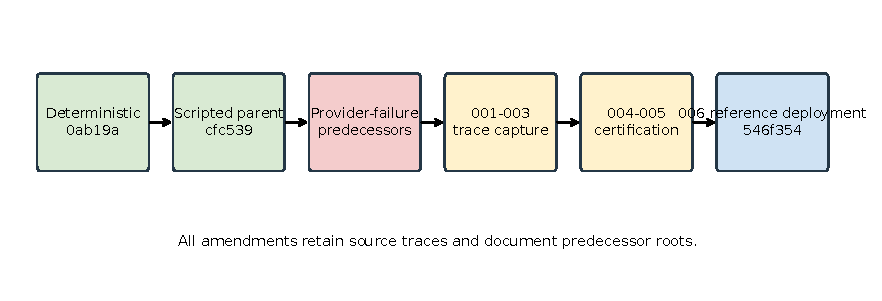
\includegraphics[width=\textwidth]{artifact-lineage}
\caption{Artifact and amendment lineage. Short prefixes identify roots; the source-verification report records full digests and predecessor links.}
\label{fig:lineage}
\end{figure*}
